\chapter{竞价云上分布式服务的可用性与成本模型}
\label{cha:jupiter}

\section{本章概述}
\label{sec:jupiter_intro}
云计算平台中广泛采用虚拟机的形式向用户提供计算资源。一个运行中的虚拟机通常被称为一个虚拟机实例。在Amazon Elastic Cloud Computing(Amazon EC2)平台中,一个支持按需付费计价方式的虚拟机实例被称为按需实例。相比于在机房中搭建物理集群,使用云平台中的按需实例能大幅度节省计算成本。许多用户包括创业团队、中小型公司以及学术研究机构等都大量使用云计算服务。从另一个层面看,底层集群架构的运行和维护成本是相对固定的,云计算服务提供商也愿意通过出租更多的计算资源提高自己的收益。

为了进一步提升资源使用率,Amazon EC2近年来推出了一种新型虚拟机实例--竞价实例(Spot Instance)。Amazon EC2对于这种新型计算实例的介绍如下:``竞价实例向用户提供了为所需的Amazon EC2云计算资源定价的方式。用户只需简单地对空闲的Amazon EC2空闲的云计算实例给出竞价,只要竞价不低于该类型计算实例的市场价格即可马上运行、使用该计算实例。竞价节点的市场则是根据市场供需关系不断变化的。''从云平台提供者的角度看,该举措能继续提升空闲计算资源的使用率。对于云租户来说,竞价实例更加便宜能够大大节省成本实现经济计算。然而,正如云平台对竞价节点的介绍所述,竞价实例不能被认为是一直可用的。无论实际环境中底层硬件的可用性多好,竞价实例都可能因竞价低于该类型节点的市场价格而被云平台回收导致不可用。这对部署在竞价节点上的分布式服务的可用性分析是一个新的挑战。

在分布式计算中,一些基础的服务被认为必须是高可用(High Availability)的。分布式锁服务是一个常见的例子。作为许多分布式应用的基础组件,分布式锁服务必须一直处于可用状态。任何锁服务的失效将导致整个分布式系统的无法运行。另一个例子是分布式存储服务,一个提供数据存储的基础组件。这些服务通常被认为是十分关键的,应该尽可能可靠。它们不同于可以在失效真正发生后进行修复的并行批处理任务\cite{Liu:2011:CMC:2170444.2170450, 5975137, Yi:2010:RCS:1844768.1845343}。对于一些关键服务,安全性必须在任何时候首先得以保证,如:一个互斥锁不能分配给多余一个申请者。这样的服务通常都有它们自身的容错机制,如:基于Paxos的状态机副本机制(State Machine Replication)。只要系统中的大多数节点在足够长的一段时间内可用,这些被应用的算法在保证正确性的同时能够保证进展性(不发生活锁,设定的目标最终达成)。

既然一个基于Paxos的容错机制可以容忍一个分布式服务中任何非大多数的节点失效,能否通过用竞价节点替换原有按需节点来提供同样高可用的分布式服务呢?用同样数量(或是更多)的竞价节点替换一个分布式系统中的按需节点非常简单,但分析这样一个分布式系统是否能提供同之前按需节点同样可用性级别的服务以及其实际的可用性则不是那么容易。新型竞价节点特有的竞价不足失效(out-of-bid failure)让分布式服务的可用性分析变得十分复杂。同传统分布式系统模型不同,节点失效概率不再是固定的一个很小的常数。因此,传统的用可容忍失效节点数来标明分布式系统可用性级别的方式需要通过引入概率失效模型加以修正。

综上,使用竞价节点提供分布式服务同时保证和使用按需节点相同的可用性级别是一个新的挑战。本章先提出了基于竞价节点的分布式系统可用性的形式化模型,然后基于该模型提出了一个针对此类分布式服务的竞价框架。该竞价框架能够根据竞价节点市场价格变化自动给出竞价决策以保证设定的系统可用性级别,同时节省分布式服务的成本。

使用易错的竞价节点构建高可用的分布式服务是可以实现的。以分布式锁服务为例,使用5个物理隔离的Amazon EC2按需计算实例构建的一个分布式锁服务在一个月内的故障停机时间一般少于30秒。\footnote{根据Amazon EC2的Service Level Agreement(SLA),按需计算实例的可用性不会低于99\%,否则使用者将获得相当于付费30\%的赔偿。由于来自不同的地理位置,5个按需计算实例是失效独立的。分布式锁服务的可用性可以通过将100\%减去任意3个或更多的节点同时不可用的概率计算得到。}。要使用竞价计算实例达到相同的可用性,可能需要7个甚至更多的竞价计算实例。具体的竞价节点个数的选择应基于对分布式服务可用性的分析。分布式服务的可用性则由每个竞价实例的失效概率决定。由于有大量的竞价策略能够满足服务可用性需求,如何选择成本最优的竞价方案是竞价框架要解决的一个问题。这个问题可以形式化为一个非线性规划问题。其目标是最小化构建分布式服务所需的竞价实例成本。其主要约束是保证同按需计算实例构成的同一分布式服务相同的可用性级别。以某一竞价申请的竞价计算实例的失效概率是相关于竞价实例市场价格的。如果用户竞价低于Amazon EC2的竞价实例市场价格,相应的竞价实例将不可用。由于竞价实例市场价格的历史序列满足马尔可夫性但价格间逗留时间在统计推断上不满足无记忆性,这里采用半马尔科夫(semi-Markvian)过程作为竞价计算实例的失效概率模型。

显然,解这样一个非线性规划是NP-hard的。在需要快速求解的情况下,使用穷举搜索法获得最优解是不实用的。本章给出了一个保证可用性的同时得到近似最优成本的用竞价节点部署分布式服务的竞价框架。该竞价框架主要有两部分组成:一个是给出竞价方案的在线竞价模块,一个是预测失效概率的竞价实例失效模型。在线竞价模块使用基于枚举和贪心策略的算法作出竞价决策。竞价实例失效模型不断地收集竞价实例的市场价格数据,并预测竞价实例在下一个时间段(如:一小时)在指定竞价下的失效概率。

\section{分布式系统的可用性}
\label{sec:jupiter_dist_basis}
副本状态机(SMR)是分布式服务实现高可用性(HA)的常见手段。SMR的容错方式是在初始状态相同的多个节点上复制执行相同的操作序列,客户端请求将被分散到多个服务器副本上。每一个操作是由副本状态机确认所有副本已达成一致。Paxos \cite{lamport2001paxos}协议已经被证明是一个高效的分布式系统一致性协议。Paxos系列协议被广泛用于实现副本状态机以构建各类高可用分布式服务 \cite{Bolosky:2011:PRS:1972457.1972472, Burrows:2006:CLS:1298455.1298487, Mu:2014:PME:2600212.2600218}。

事实上,Paxos是一种基于Quorum投票方式\cite{Gifford:1979:WVR:800215.806583}的分布式系统一致性达成机制。这类协议通常采用类似投票的算法,一个请求必须获得足够多的节点投票$v$才能够执行一个操作。一个可行的$v$值称为Quorum。只要有足够的可用节点投票,分布式系统就是可用的。否则,由于可用节点没有足够的投票,整个系统被视为不可用的。

服务可用性可以被定义为请求获得合理响应的概率。一个分布式服务的可用性由其分布式系统中各个节点的失效概率决定。文献\cite{Peleg1995210}研究了基于法定人数的分布式系统可用性。便于讨论起见,这里先引入可接受集(Acceptance Set)的概念\cite{Amir1998223}。

\begin{definition}
代表分布式系统节点的有限集$U$上的一个集合$\mathcal{A}$满足如下条件时可以称之为一个可接受集:
\begin{enumerate}[1)]
\item 对于所有$S, T \in \mathcal{A}$,$\cap T \neq \emptyset$。
\item 如果$S \in \mathcal{A}$,则对于所有$T \supseteq S$,$T \in \mathcal{A}$。
\end{enumerate}
最小Quorum集合为$\mathcal{S}$ = $\mathcal{S}(\mathcal{A})$ = $\{S \in \mathcal{A} \mid S \setminus \{u\} \notin \mathcal{A}$,$\forall u \in S\}$.
\end{definition}

假设$\mathcal{A}$为一个分布式系统的一个可接受集,对于每一个集合$S \in \mathcal{A}$,集合$S$中的所有节点都正常运行而其余节点都失效的概率是
\begin{equation}\nonumber
\prod_{i \in S} (1-p_i) \prod_{j \in \overline S} p_j,
\end{equation}

其中,$\overline S$表示$U \setminus S$,$\bf p$ $= (p_1, p_2, \cdots, p_n)$表示分布式系统中各个节点一段时间内的失效概率。

由于$S$代表所有可接受集,$\mathcal{A}$的非失效概率亦即可用性可进一步表示为:
\begin{equation}\label{eq_a_as}
A_{\mathcal{A}} = \sum_{S \in \mathcal{A}}(\prod_{i \in S} (1-p_i) \prod_{j \in \overline S} p_j)
\end{equation}

在此,我们引入另一个定义:\emph{最优可接受集}。
\begin{definition}
代表分布式系统节点的有限集$U$上的一个可接受集$\mathcal{A}$可称之为最优可接受集,当:
\begin{enumerate}[1)]
\item 对于在相同集合$U$上的所有可接受集$\mathcal{B}$,有$A_{\mathcal{A}} \geq A_{\mathcal{B}}$。
\end{enumerate}
\end{definition}

对于一个分布式系统,其最优可接受集的非失效概率 $\mathcal{A}_{o}$ 等价于其上的分布式服务的可用性期望。这里讨论的可接受集假设各个竞价计算实例之间失效独立。这和我们之前提到的将高可用服务部署在不同可用区(Availability Zones)的计算实例上的讨论是相一致的。通过一个分布式系统最优可接受集的可用性期望,我们可以给出该系统上的分布式服务的可用性估计。该估计可用于构成将在后文中详细讨论的非线性规划模型中的主要约束条件。

\section{可用性与成本优化问题的形式化}
\label{jupiter-formulation}
因为在分布式系统中配置基于Paxos的副本状态机(SMR)可以容忍任意的少于一半数量的节点同时失效问题,似乎我们直接将分布式系统中部署于竞价计算实例之上。事实上,这并不能保证分布式服务拥有同样的可用性。这里用一个简单的例子进行解释。

假设一个基于Paxos的分布式系统有5个节点。每个节点的失效概率是0.01。这个分布式系统能容忍任意不多于两个节点的同时失效。根据公式\eqref{eq_a_as},其上的分布式服务的可用性期望是0.9999901494,这意味着该服务在一个月时间中的停机故障时间只有约25.5秒。如果将所有5个节点替换为竞价计算实例,且将竞价均设为和其市场价格相同,可用性级别将大打折扣。虽然替换节点后的分布式系统仍然能够和之前一样容忍任意不超过两个节点的同时失效,该分布式系统的非失效概率远远低于之前的配置。已2014年6月Amazon EC2平台的来自不同可用区(Availability Zones)的5个m1.small类型竞价计算实例为例,可用区US East 1a, US East 1c, US West 1b, US West 2a, US West 2b在2014年6月1日凌晨零点的市场价格分别为:0.8美分,0.8美分,0.9美分,0.9美分,0.9美分。如果我们在每个可用区以前述的价格各申请一个该类型的竞价实例组成相同的分布式系统,节点失效将较正常节点发生的更为频繁。在整个2014年6月,其上的分布式服务的故障停机时间将超过1500秒。

本质上,对于分布式系统来说,在使用竞价计算实例时能够至多容忍的同时失效节点数不能表征同使用按需计算实例同样的系统可用性。因为竞价计算实例的失效概率远高于按需计算实例。竞价实例的失效概率随着竞价实例市场价格的波动不断变化。因此,我们通过竞价和市场价来刻画竞价计算实例的失效概率。

基于竞价实例的节点失效模型,可用性与成本优化问题可抽象为一个竞价决策问题,即:如何保证分布式服务保持指定的高可用性级别,以及如何通过设定竞价最小化竞价实例的成本开销。该优化问题可通过一个非线性规划模型来描述。

\subsection{竞价计算实例失效模型}
\label{jupiter-sifm}
分布式系统的可用性基于系统中各个组件的可用性。考虑云平台中的计算实例,一个节点的可用性可以通过其失效概率估计。令$MTBF$ (Mean Time Between Failures)表示一个计算实例的两次故障的平均间隔时间, $MTTR$ (Mean Time To Repair) 表示一个计算实例从故障中恢复所需的平均时间, 云平台中的一个计算实例的可用性$A$可以按下式测得:
\begin{equation}\label{eq_a}
A = \frac{MTBF}{MTBF+MTTR}
\end{equation}

导致一个计算实例失效的原因各种各样,包括硬件、软件、电力供应等层面的错误。根据Amazon EC2云平台的服务等级协议(SLA)\cite{AWS_SLA:2014}, 一个按需计算实例测得的可用性是0.99,也就是其失效概率是0.01。

对于云平台中的竞价计算实例,不同于其它类型节点、主要的失效原因是竞价不足。其原因是竞价实例的市场价攀升到了原定竞价之上。单独考虑这一类型的节点失效,一个竞价实例在时间点$t$的失效概率可表示为:
\begin{equation}\label{eq_a_ob_instant}
Pr(p(t)>b)
\end{equation}

其中 $p(t)$ 在时间点 $t$ 的竞价实例市场价格, $b$ 当时的表示竞价。


因为在云平台中其它各种类型的失效同竞价不足导致的失效是不相关的,且一个竞价实例在不发生竞价不足导致的失效时同按需节点可用性相同,一个竞价计算实例的失效概率 $FP(t)$ 可以进一步表示为:
\begin{equation}\label{eq_a_instant}
FP(t) = 1 - (1 - FP^{\prime}) \cdot (1 - Pr(p(t)>b))
\end{equation}

其中 $FP^{\prime}$ 表示相对应的按需计算实例的失效概率,这里 $FP^{\prime} = 0.01$。

一个竞价计算实例在一个时间段 $d, d>0$ 的失效概率可以进而表示为:
\begin{equation}\label{eq_fpd}
\int_0^d FP(t)dt
\end{equation}

竞价云平台以所有竞价者用户的竞价降序作为排序依次向竞价用户分配竞价实例。直到所有可用的竞价实例已被分配完或所有用户的竞价实例请求已经被满足。竞价实例的市场价格等于获得竞价实例的最低用户竞价。一段时间后,竞价实例的市场价格可能根据整个市场的供给和需求发生改变。图 \ref{figure:sil} 描绘了2014年6月24日 上午9点到11点``us-east-1''可用区``linux.m1.small''类型竞价实例的市场价格历史数据。其市场价格在切换为0.81美分/小时之前先停留在0.71美分/小时,半个小时后上升为1.17美分/小时。估计一个竞价实例的失效概率应基于竞价实例的市场价格波动。

\begin{figure}
  \centering
  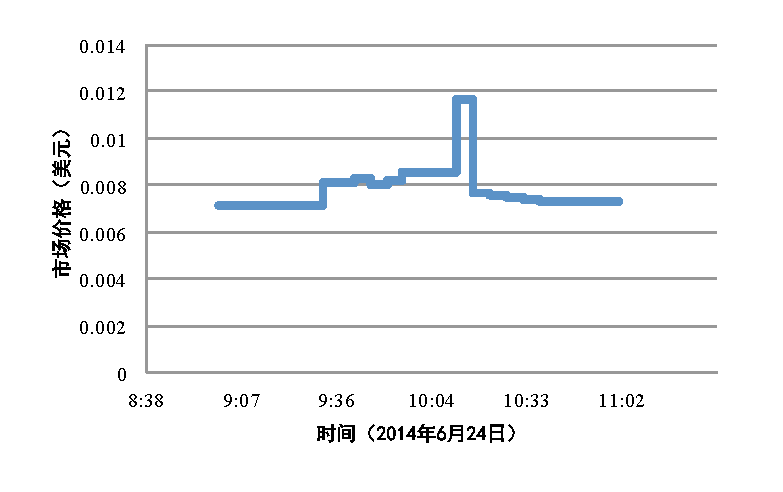
\includegraphics{SpotPrice}
  \caption{一个``us-east-1a''可用区的``linux.m1.small''类型的竞价实例的市场价格历史数据}
  \label{figure:sil}
\end{figure}

如图\ref{figure:sil}所示,竞价实例市场价格在一段时间 $d_i$ 内保持在一个固定值 $S_{i}$,而后切换到一个新的值 $S_{i+1}$ 。实质上,
市场价格序列 ($S_i, i = 1, 2, \cdots, n$) 和逗留时间序列 ($d_i, i = 1, 2, \cdots, n$) 都可用随机过程来描述. 已有研究工作\cite{chohan2010see} 通过验证Chapman-Kolmogorov 等式 \cite{grimmett1992probability}证明市场价格序列满足马尔科夫性。而逗留时间序列可以用一个时序点过程来描述 \cite{eltit}。

由于市场价格之间的逗留时间不满足无记忆性,市场价格的变化可刻画为一个半马尔可夫(semi-Markovian)链模型,在文献\cite{song2012optimal}中也采用了同样的模型。将所有有效市场价格的集合表示为 $\mathcal{S}$,其中 $\mathcal{S} = \{s_i, i = 1, \cdots, \left|\mathcal{S}\right|\}$, 将所有逗留时间的状态空间表示为 $\mathcal{T}$,其中 $\mathcal{T} = \{\tau_i, i = 1, \cdots, \left|\mathcal{T}\right|\}$。该半马尔可夫链的随机核(Stochastic Kernel)可表示为:
\begin{equation}
Q(i, j, k) = (q_{i, j, k}; s_i, s_j \in \mathcal{S}, k \in \mathcal{T})
\end{equation}

其中,
\begin{equation}
q_{i, j, k} = Pr(S_{n+1} = s_j, S_n = s_i, \tau_n = k)
\end{equation}

即,状态 $i$ 在时间后 $k$ 转移到状态 $j$ 的概率。

详细的统计推断参见\cite{song2012optimal}。通过这个竞价实例市场价格模型,我们可以计算未来一段时间两个市场价格间发生转移的概率,进而估计在给定竞价下一个竞价实例的在未来一段时间的失效概率。

\subsection{成本最小化问题}
竞价决策可以抽象为一个非线性规划模型。目标是最小化构建分布式服务的竞价成本。约束是使用竞价实例部署的分布式服务的可用性不差于使用按需实例部署的同一服务。分布式服务的可用性估计基于竞价实例的失效概率。

根据前文介绍的竞价云平台的定价规则,用户无需支付因云平台回收机器造成的不足一小时部分的开销。如果一个用户能够精确竞价实例的价格变化,利用这个特点减少计算成本甚至是零成本计算是可能的。然而,精确预测何时发生价格变化以及变为什么价格是非常困难的。利用竞价不足失效免费使用云计算资源看似美好,实则基本不可行。本文无意去探讨利用竞价云平台的这类竞价实例定价规则,以简化使用竞价实例部署分布式服务的成本最优化问题。

在竞价云平台中,不同的可用区不仅隔离了各种计算实例的硬件、软件错误,而且隔离了竞价不足失效。不同可用区竞价实例属于不同的市场。为确保如前文所述的申请的竞价节点的失效独立性,分布式服务在每个可用区应该至多申请一个竞价实例。以Amazon EC2竞价云平台为例,共有超过20个可用区。这对于选出组成一个实际系统中的Paxos组的节点规模(通常为5或7个节点)\cite{Burrows:2006:CLS:1298455.1298487}已经足够。性能需求可通过运行多个Paxos组加以满足。

因为竞价云平台一般以小时为单位计费,竞价的周期应该设为 $n$ (一个正整数)小时。在每个竞价周期,成本最小化问题可形式化为一个非线性规划问题。在这个模型中,决策变量是用户在各个可用区给出的竞价。竞价决策可被表示为一个向量 $\bf b$ $= (b_1, b_2, \cdots, b_n)$. 其中,在第$i$个可用区申请竞价实例的竞价为 $b_i$, $i = 1, 2, \cdots, n$。

当进行竞价时,下一个小时申请到的竞价实例的开销仍然是未知的。这是因为竞价云平台的计费是以该小时的最后一个市场价格作为计费价格,而不是用户申请时给出的竞价。对于一个由多个竞价实例组成的系统,目标是各个竞价实例的成本之和最小。由于未来时间点的竞价实例市场价格是一个随机变量,我们这里使用竞价实例的竞价之和作为非线性规划的目标函数。显然竞价之和是实际成本之和的一个上界,通过最小化竞价之和可以严格控制成本。

非线性规划模型中的关键约束是确保使用竞价实例部署的分布式服务有和使用按需实例部署的同一服务有相当的可用性。分布式服务的可用性可被表示为其最优可接受集的可用性。这里将一个分布式服务 $S$ 的最优可接受集表示为 $\mathcal{A}_{o}(S, \bf{FP})$,其中 $\bf{FP}$ 竞价实例节点失效概率向量。 将一个使用竞价实例部署的分布式服务表示为 $S_s$, 第 $i$ 个可用区的某类型竞价实例的市场价格表示为 $p_i$,服务 $S_s$ 中使用的各个可用区的竞价实例在指定竞价 $\bf b$ =$ (b_1, b_2, \cdots, b_n)$ 下的节点失效概率为 $FP(\bf b)$。类似的,将一个使用按需实例部署的对应分布式服务表示为 $S_o$,在使用按需实例部署的服务 $S_o$ 中按需实例节点个数为 $m$。成本最优化问题最终可形式化为:
\begin{equation}
\min \sum_{i=1}^n b_i
\end{equation}
s.t.
\begin{equation}\label{eq_bgp}
\sum_{i=1}^n {\epsilon(b_i - p_i)} \geq m
\end{equation}
and
\begin{equation}\label{eq_aae}
A_{\mathcal{A}_{o}(S_o, {\bf{FP^{\prime}}})} - A_{\mathcal{A}_{o}(S_s, FP(\bf b))} < \varepsilon
\end{equation}

其中,不等式 \eqref{eq_bgp} 是一个基本约束,开始时有足够的节点在线以保证使用竞价实例部署的分布式服务能够初始化正确。在不等式 \eqref{eq_aae} 中, $\epsilon$(u) 为一个 $u$ 是否大于0的判定函数,$\varepsilon$ 表示一个无穷小量。在实际使用汇总,可以将其设置为一个可接受的可用性误差,如 0.000001。

\section{竞价框架及策略}
\label{jupiter-framework}
解决上述非线性规划问题是NP-hard的。需要遍历所有可能的竞价 $\bf b$ 验证其是否满足可用性约束。遍历空间的大小是 $m^n$,其中 $m$ 是可能的价格数,而 $n$ 不同的可用区个数。显然,枚举搜索的方法是不能实际应用的。

幸好,从用户角度来看,意图是减少竞价实例的使用成本而不必获得最优解。既然在可接受的短时间内求得最优解是不可能的,不妨退而求其次获取一个接近最优解的竞价决策。下面主要介绍能够实际应用的成本和可用性感知的使用竞价实例构建分布式服务的竞价框架。如图 \ref{figure:framework} 所示,竞价决策在每个竞价周期的开始由在线竞价模块给出。然后竞价实例申请被发送给竞价云平台。竞价实例节点失效预测模块用于估计在下一个竞价周期中一个竞价实例在指定竞价下的失效概率。估计的竞价实例失效概率用于验证整个分布式系统的可用性需求约束。随着不断采集竞价实例市场价格数据,竞价实例的失效概率的预测可以得以改善。
\begin{figure}
  \centering
  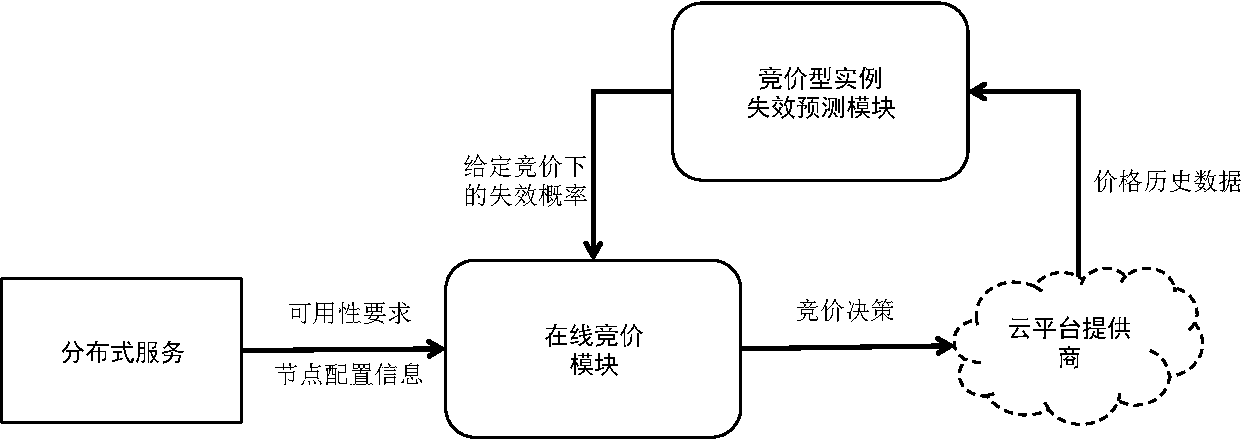
\includegraphics[width=1.0\textwidth]{CAB_arch}
  \caption{竞价框架}
  \label{figure:framework}
\end{figure}

在这个竞价框架下,如果竞价实例市场价格大幅变动,在新的竞价周期竞价决策将随着发生改变。一些竞价实例需要被替换为其它可用区的竞价实例。为保证节点替换过程中服务的可用性,新加入的竞价实例在新的竞价周期开始之前就被启动并加入到分布式系统中,然后被替换的节点在新的竞价周期开始时被移除。加入和移除竞价实例可以通过Paxos的视图切换(View Change)操作完成。一个竞价实例的启动时间通常需要200秒或更多,在不同云平台的区域有一些差别\cite{Mao:2012:PSV:2353730.2353859}。因此,一个竞价周期的实际时间有所减少。后文中将对不同竞价周期的选取进行讨论。

\subsection{在线竞价算法}
\label{subsec:jupiter-bidding}
如前文所述,在一个传统的分布式系统模型中节点的失效概率是固定的,通常为一个非常小的常数。法定投票数(Quorum)就是简单的分布式系统中所有节点的大多数。对于分布式系统中的节点失效概率各不相同的情况,基于权重的投票权分配方法已经被证明是最优配置。基于权重的最优可用性投票权分配机制已在文献\cite{25789, 262589, Amir1998223}中得到很好的研究。这里将所有$n$个节点的失效概率表示为 $p_i, i = 1, 2, \cdots, n$。文献\cite{Amir1998223}已经证明:如果 $p_i \geq \frac{1}{2}, \forall i$, 最优投票权分配方式不再是民主式的相同投票权重,而是所有节点中相对可靠性最高的节点拥有绝对权重即由该节点集权。如果系统中只有部分节点 $i$ 满足 $p_i \geq \frac{1}{2}$, 在一个最优投票分配中所有这些失效概率大于 $\frac{1}{2}$ 的节点不应该得到投票权。如果 $0 < p_i < \frac{1}{2} \forall i$,最优投票权重可由下式 \cite{262589, 25789}给出:
\begin{equation}\label{eq_ow}
w_i = log_2(\frac{1-p_i}{p_i})
\end{equation}

然而,在一个实际使用场景中,公式 \eqref{eq_ow} 在各个节点失效概率差异较大的情况下不能被直接应用。例如:一个有三个节点的分布式系统中节点失效概率分别是:0.01,0.1,0.1。根据公式 \eqref{eq_ow},节点失效概率为0.01的节点拥有占支配地位的投票权,超过了另外两个节点的投票权之和。这在理想情况下是合理的,因为当一个节点的可靠程度远远高于另外两个节点时由它来决定系统可用性是最优的。但在实际情况下,节点的失效概率是在有限时间段内估测出的,与无限时间下平稳态的理想值有一定的偏差。竞价实例失效模型中的竞价不足失效正是这样一种情况。另外,一些Paxos系列的协议在设计过程中并未考虑投票权重不同的情况。为保证竞价算法简单性和兼容性,维持Paxos中的简单大多数投票方式是必要的。

由于每个竞价实例被固定分配了相同的投票权,根据最优投票权分配方式各个竞价实例应有相同的失效概率。在本文的在线竞价算法中,各个竞价实例的失效概率会趋近于相同。该算法使用了枚举和贪心的策略。

\begin{figure}
\rule[-.2pt]{\textwidth}{0.9pt}
\textbf{Algorithm: Bidding}

\rule[-.2pt]{\textwidth}{0.5pt}

\begin{algorithmic}[1]
\Require{$availability$, $type$}
\Ensure{$bids$}

\State $zones\gets get\_availability\_zones()$
\State $n\gets 1$
\While{$n \not> zones.length$}
    \State $FP\gets node\_failure\_pr(n, availability)$
    \ForAll{$zone \in zones$}
        \State $spotprice\gets get\_spot\_price(zone, type)$
        \State $bid\gets spotprice.price$
        \While{$bid \not> get\_on\_demand\_price(zone, type) $}
            \If{$estimate\_FP(zone, bid, spotprice) \not >FP$}
                \State $\textbf{break}$
            \Else{}
                \State $bid\gets bid + 1$
            \EndIf
        \EndWhile
        \State $bids[n][zone]\gets bid$
    \EndFor
    \State $sort(bids[n])$
    \State $cost\_upper\_bound[n]\gets sum(bids[n][1:n])$
    \State $n\gets n + 1$
\EndWhile
\State $m\gets min\_key(cost\_upper\_bound)$
\State \Return{bids[m][1:m]}
\end{algorithmic}
\rule[-.2pt]{\textwidth}{0.8pt}
\caption{在线竞价算法}\label{figure:bidding-algo}
\end{figure}

在线竞价算法伪代码如图 \ref{figure:bidding-algo} 所示。该算法接受一个分布式系统配置信息作为输入,包括系统可用性和节点类型需求等。整个在线竞价步骤简单:1)对于所有可能的节点数 $n$,计算在各个节点失效概率相同情况下的满足系统可用性要求的节点失效概率最大可能值 $FP$。2)在 $n$ 个节点的配置下,对于所有可用区计算估计失效概率小于 $FP$ 的最小竞价。预测的失效概率依赖于各个可用区的竞价实例失效模型、竞价、竞价实例市场价格、市场价格逗留时间。3)比较所有可用区的竞价值,以贪心的方式选择可用区。4)累加所选择的可用区竞价,计算在每一个节点数配置下计算成本的上限并返回成本上限最小的竞价方案作为竞价决策。这个算法不能保证总是给出一个最优的竞价决策,但在实际使用中能给出一个接近最优的竞价方案。

\subsection{失效概率预测}
在竞价框架中,在线竞价模块需由竞价实例失效模型完成各个竞价实例节点失效概率的预测。为估计竞价实例的失效概率,竞价实例的市场价格预测模型被嵌入到竞价实例失效模型中。如前文中 \ref{subsec-sifm} 节所述,竞价实例的市场价格的变化被形式化为一个半马尔科夫链模型。因此,竞价实例失效概率预测的一个关键任务是从观测中的竞价实例市场价格历史数据中重新构造出概率转移分布。
研究者Wee\cite{5948651}在2011年认为竞价实例市场价格采样累计分布函数约每一个小时有明显的增长。然而,收集到的2014年竞价实例市场价格数据显示市场价格的变化频率已经加快为每小时多次。简单起见,这里将半马尔可夫链的时间单位设置为1分钟,采样数据中的逗留时间 $d_i$ 被离散化为
\begin{equation}
\tau_i \triangleq \tau(S_i \rightarrow S_{i+1}) \triangleq \lfloor d_i \rfloor
\end{equation}

这里采用一个经验估计方法,本质上类似于极大似然估计(Maximum Likelihood Estimator) \cite{Barbu:2008:SCH:1481376}。统计核(stochastic kernel) \textbf{Q} 被重构为:
\begin{equation}
\widehat{{q}_{i,j,k}} = \frac{N_{i, j}^{k}}{N_i}, \forall N_i \neq 0
\end{equation}

当$N_i = 0$时,$\widehat{{q}_{i,j,k}} = 0$。

其中,$N_i$ 价格 $s_i \in \mathcal{S}$在采用中的出现次数,$N_{i, j}^{k}$ 表示价格在逗留时间 $k \in \mathcal{T}$ 从 $s_i \in \mathcal{S}$ 转移到价格 $s_j \in \mathcal{S}$ 的次数。

竞价最高可以设置为同类型按需实例的10倍,当竞价实例的市场价格高于同类型按需实例时,应选择选择按需实例以避免高昂的竞价计费。因此,在本文的竞价框架中一个合法的竞价不应超过其对应类型的按需实例,价格等于对应按需实例价格的竞价视为申请一个按需计算实例。在一个时间单元,竞价实例在指定竞价下的失效概率为
\begin{equation}
FP(b) = 
\begin{cases}
1 &\mbox{if $0 \leq b \leq p$}\\
1 - (1 - FP^{\prime}) \cdot \sum\limits_{j=p}^b{\widehat{{q}_{p, j, k}}} &\mbox{if p < b < o}
\end{cases}
\end{equation}

其中 $b$ 表示一个竞价,$p$表示竞价实例市场价格,$k$ 表示逗留时间,$o$ 表示对应类型的按需实例价格,$FP^{\prime}$ 表示对应按需实例的失效概率,为一个固定值0.01。

竞价实例在一个竞价周期的失效概率是其在每个时间单元的失效概率期望,即公式 \eqref{eq_fpd} 的离散形式。

\section{系统评测}
\label{sec:jupiter-evaluation}
基于前述竞价框架设计,本章的工作还包括用Python实现了一个面向Amazon EC2云平台的竞价框架原型Jupiter。该竞价框架通过亚马逊云服务(Amazon Web Services)Python接口库 \emph{boto} \cite{boto:2014} 同Amazon EC2交互。为全面评测我们的竞价框架,我们将其用于部署在Amazon EC2上的一个分布式锁服务和一个分布式存储服务。整个实验包括一个微基准测试,一个一周时间的运行于Amazon EC2的可行性验证测试,和两个11周时间的基于价格纪录重放的成本和可用性评测。

\subsection{实验用分布式系统}
\label{subsec:jupiter-bc}

\subsubsection{分布式锁服务}
\label{subsection-case-dls}
分布式锁服务一般用于松耦合的分布式系统中。一个代表性的分布式锁服务是 \emph{Google Chubby} \cite{Burrows:2006:CLS:1298455.1298487},可用于数千个节点的活动同步以及基本信息确认,例如:系统成员信息。

\emph{Chubby} 提供了一个非常像文件系统的建议锁(Advisory Lock)的接口,并使用Paxos作为生产环境下的分布式一致性协议以保证高可用性。一个Chubby服务器通常配置成5个副本。Chubby客户端通过使用RPC调用库实现和Chubby服务器的通信。这样五个节点组成的分布式系统的投票方式采用简单多数原则。Chubby遵循不同副本部署于不同区域(和Amazon EC2等云平台的可用区概念相似)的假设。

\subsubsection{基于纠删码的分布式存储服务}
\label{subsubsec:dss}
分布式存储服务通常为客户端提供对象存储或键值存储,可容忍部分节点的暂时性故障甚至是永久性的机器和磁盘损坏。在多个可用区间构建分布式存储服务可以容忍数据中心故障或网络中断以提供更好的可用性。不同于主从式技术,Gaios \cite{Bolosky:2011:PRS:1972457.1972472} 和 Megastore \cite{baker2011megastore} 已在分布式存储服务的实现中采用了基于Paxos的状态机副本(SMR)机制进行容错。

纠删码 \cite{Rizzo:1997:EEC:263876.263881} 是一种信息理论中的前向错误纠正编码方式,原本用于在网络通信中独立数据包丢失的情况下进行消息恢复,现已广泛用于分布式存储系统 \cite{Huang:2012:ECW:2342821.2342823, Sathiamoorthy:2013:XEN:2488335.2488339},用于减少存储和网络开销。在一个通常形式的纠删码编码中,原始数据通常被划分为$m$个大小相同的数据块,然后计算并生成$k$个大小相同的校验块,数据块的总数是 $n = m + k$。纠删码算法能够从 $n$ 个数据块中的任意 $m$ 个数据块重构出原始数据。这样的一个纠删码编码可以表示为 $\theta (m,n )$。

近来,Mu等研究者 \cite{Mu:2014:PME:2600212.2600218} 提出了一个Paxos协议的变体,RS-Paxos,可以在没有同步(Synchronous)网络模型的前提下实现分布式系统中基于纠删码的一致性决议。RS-Paxos可被用于分布式存储系统,通过在各个节点上发送编码后的数据块而不是全部数据拷贝大大减少了网络数据传输和磁盘数据写入。这样的分布式服务被称为基于纠删码的分布式服务。

一个标准的RS-Paxos配置是5个节点,纠删码编码方式为 $\theta(3, 5)$。需要注意的是,这里RS-Paxos最多仅能容忍一个节点失效而不是两个节点失效。这和上一节中的分布式锁服务是非常不同的。这是因为基于纠删码的分布式存储服务中写入操作所需的法定投票数不同于各个节点间数据全副本的方式。为保证能够重构出原始数据,可接受集的交集(Intersection)大小应该是3,而不是1。

\subsection{实验设置}
使用按需实例部署的上述两个分布式服务被设置为我们后续实验中的基线。虽然使用预留计算实例可以至多减少30\% $\sim$ 40\% 的成本,由于其不灵活性以及难于适应变化的服务负载,本实验中不再加以比较。根据Amazon EC2云平台的文档\cite{AWS_SLA:2014},一个按需计算实例的失效概率被设定为0.01。实验中用到的分布式锁服务是一个基于Paxos的简单实现,分布式存储服务是一个基于RS-Paxos的实现\cite{Mu:2014:PME:2600212.2600218}。在这两个系统中节点数都配置为5,这是实际生产系统中的通常配置\cite{Burrows:2006:CLS:1298455.1298487, Mu:2014:PME:2600212.2600218}。在这样一个配置中,分布式锁服务能够容忍任意不超多两个节点失效。如前文\ref{subsubsec:dss}节所述,分布式存储服务则只能容忍至多一个节点失效而不是两个节点失效。

实验中使用了一个启发式的竞价策略作为对照组。假设原有使用按需计算实例的分布式系统中 $n$ 个节点,该策略选择竞价实例市场价格最低的 $n + m$ 个可用区申请竞价实例,$m$ 为该策略使用的额外节点数。对于每个被选出的可用区,该策略给出的竞价为竞价实例的市场价格加上一个额外的溢价比例 $p$,如:10\%或20\%。由于有大量的 $m$ 和 $p$ 可供选择,实验中使用了一些有代表性的 $m$ 和 $p$ 用于比较实验结果。方便起见,有 $m$ 个额外节点和超出竞价实例市场价格比例 $p$ 的启发式策略后文中将表示为 $Extra(m, p)$。

实验使用了Amazon EC2云平台的17个可用区。分布式锁服务采用``linux.m1.small''类型实例部署,每个该类型实例在各个可用区的价格有所差别,大约为4.4 $\sim$ 6.1美分/小时。基于纠删码的分布式存储服务使用``linux.m3.large''类型实例构建,该实例类型相比``linux.m1.small''类型拥有更多的计算资源和内存容量。每一个该类型按需实例的价格在各个不同可用区约为 14 $\sim$ 20.1 美分/小时。

对于每一个可用区,竞价实例失效模型使用大约三个月的竞价实例市场价格历史数据进行训练。从训练的结果上看,模型已经趋于收敛。在整个实验过程中,我们在Amazon EC2云平台上使用竞价框架运行分布式锁服务和基于纠删码的分布式存储服务约一周时间。然后,根据Amazon EC2的竞价实例计费规则重放了两个11周长的竞价实例市场价格数据仿真了前述两个分布式服务在不同竞价框架下的运行。在仿真中,竞价实例的启动时间已经加以考虑。竞价实例启动时间在不同区域间有很大不同,通长在200 $\sim$ 700秒之间\cite{Mao:2012:PSV:2353730.2353859}。

\subsection{微基准测试}
对于竞价实例失效模型,需要重点关注的是其对竞价实例失效概率的预测精度。据此,在微基准测试中需要比较测得的竞价实例失效概率和模型预估的竞价实例失效概率期望。测试中采用了一种间接的比较方式:先使用竞价实例失效模型模型确定各个可用区竞价不足失效概率在一个月时间内不超过0.01的竞价,然后通过比较竞价和该月的竞价实例市场价格数据计算实际的竞价不足失效概率。通过比较实际的竞价不足失效概率和0.01可以得出模型预测的大致可靠程度。图\ref{figure:fp}显示了在5个可用区的竞价不足失效概率。
\begin{figure}
  \centering
  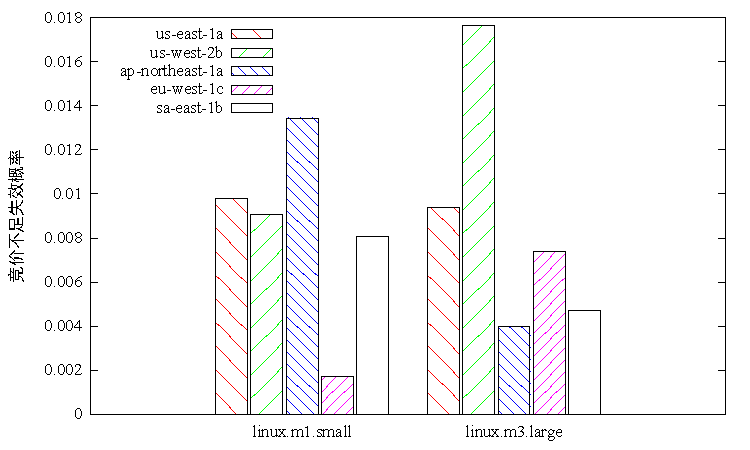
\includegraphics[width=1.0\textwidth]{fp}
  \caption{预估竞价不足失效概率为0.01竞价下的实际失效概率}
  \label{figure:fp}
\end{figure}

对于``linux.m1.small'' 和 ``linux.m3.large'' 两种类型的竞价实例,大部分情况下测得的竞价不足失效概率都小于0.01。在所有测试中有两个略大于0.01的例外:一个是在``ap-southeast-1a''可用区,针对``linux.m1.small''类型竞价实例的竞价不足失效概率约为0.013553;另一个是在``us-west-2b''可用区,针对``linux.m3.large''类型的竞价实例的竞价不足失效概率为0.017665。测试结果表明竞价实例失效模型可以在一个较小误差内估计失效概率。

\subsection{可行性验证}
在2014年12月,竞价框架在Amazon EC2云平台上进行了长达一周的运行测试。使用Jupiter框架运行正确,在一周时间内保证了两个分布式服务一直可用。使用$Extra(0, 0.1)$启发式策略的框架作为对照组也同时运行。两个竞价策略中的竞价周期均设为1小时。
\begin{figure}
  \centering
  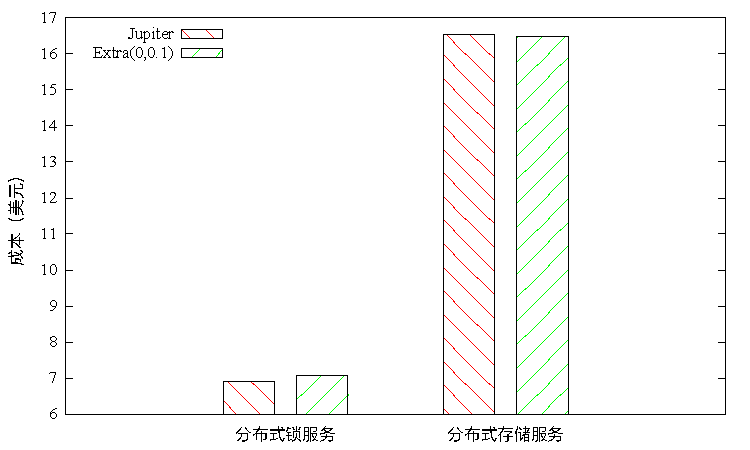
\includegraphics[width=1.0\textwidth]{rr}
  \caption{不同竞价策略下的竞价计算实例成本(2014年12月15-22日)}
  \label{figure:rr}
\end{figure}

如图\ref{figure:rr}所示,在一周的运行中,Jupiter竞价框架下分布式锁服务的计算成本约为6.91美元,只有使用按需计算实例的六分之一左右,也略低于 $Extra(0, 0.1)$ 竞价策略的成本。两个竞价策略在一周的运行中,分布式锁服务一直处于可用状态。相应地,分布式存储服务使用Jupiter竞价框架运行一周的计算成本是16.53美元,同使用 $Extra(0, 0.1)$ 策略的成本相近。在可用性方面,Jupiter竞价策略保证了分布式存储服务在一周的运行中一直可用,而 $Extra(0, 0.1)$ 策略则出现了一次竞价不足失效导致的服务不可用。总的来看,Jupiter竞价框架在可用性和成本上要好于用于对照的启发式竞价策略。实验结果表明,Jupiter竞价框架可在显著减少计算成本的同时保证使用竞价实例部署的分布式服务高可用。

\subsection{成本和可用性评测}
\label{subsec:ca}
本节通过对长期的竞价实例市场价格历史数据重放仿真对竞价框架进行评测。因为仿真实验中一个竞价实例的开销和可用性均由给定的竞价实例市场价格数据确定,仿真结果同在Amazon EC2平台中运行竞价框架的结果是相同的。两个启发式策略 $Extra(0, 0.2)$ 和 $Extra(2, 0.2)$,也进行了相同的仿真实验作为对照。在仿真实验中,所使用的数据包括2014年10月至12月间的 ``linux.m1.small'' 类型和 ``linux.m3.large'' 类型竞价实例的市场价格历史数据。其中,分布式锁服务的仿真实验使用 ``linux.m1.small'' 类型竞价实例的市场价格数据,分布式存储服务的仿真实验采用 ``linux.m3.large'' 类型竞价实例的市场价格数据。评测主要关注两个分布式系统部署案例中服务的可用性和成本。竞价周期除了1个小时外,还测试了其他几种不同的配置。

11周时间使用5个 ``linux.m1.small'' 按需实例的分布式锁服务的计算成本以最便宜的可用区计算是406.56美元。对于基于纠删码的分布式存储服务,11周时间运行5个 ``linux.m3.large'' 按需实例以最便宜的可用区计算其成本是1293.6美元。这两个值作为成本的评测基线。两个分布式服务在不同竞价策略下的成本如图 \ref{figure:dlscost} 和 \ref{figure:dsscost}所示。图 \ref{figure:dlsavailability} 和 \ref{figure:dssavailability} 给出了不同竞价策略在可用性方面的评测结果。

如图 \ref{figure:dlscost} 所示,本章提出的竞价策略在分布式锁服务的案例中只需约基线五分之一的成本。将竞价周期设为6小时获得了评测中最好的结果,计算成本约77.3美元。对于1小时,9小时以及12小时的竞价周期,本章提出的竞价策略所需成本略高于对照的启发式策略 $Extra(0, 0.2)$ 。启发式策略 $Extra(2, 0.2)$ 的成本则要明显高于其他两个竞价策略。

对于分布式锁服务的案例如图\ref{figure:dlsavailability}所示,Jupiter竞价框架除了竞价周期为12小时的配置没有发生服务失效不可用的情况(可用性接近1)。而另外两个启发式策略则无法保证相同的可用性级别。在使用对照组启发式策略 $Extra(0, 0.2)$ 时,11周中累计有8小时的时间服务处于故障停机状态。这远远达不到高可用服务的要求。在另外一个对照组启发式策略 $Extra(2, 0.2)$ 下,分布式锁服务的可用性要好于 $Extra(0, 0.2)$ 策略。但在不同竞价周期中仍然无法满足服务可用性级别的约束。
\begin{figure}
  \centering
  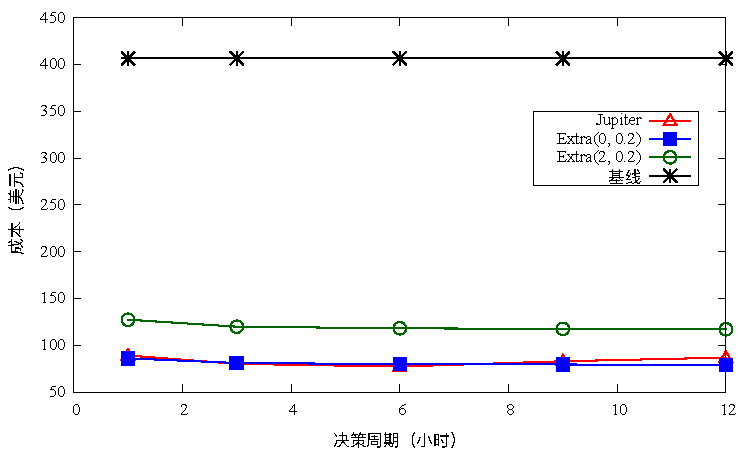
\includegraphics[width=1.0\textwidth]{cost-dls}
  \caption{不同竞价策略下分布式锁服务的竞价实例租用成本(2014年10-12月)}
  \label{figure:dlscost}
\end{figure}
\begin{figure}
  \centering
  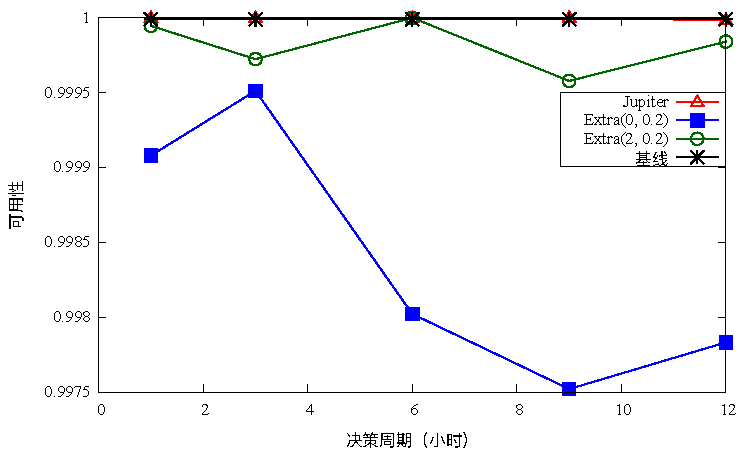
\includegraphics[width=1.0\textwidth]{ava-dls}
  \caption{不同竞价策略下分布式锁服务的可用性(2014年10-12月)}
  \label{figure:dlsavailability}
\end{figure}

对于策略 $Extra(0, 0.2)$,每个竞价周期申请的竞价实例数都是5个。而策略 $Extra(2, 0.2)$ 每次申请的竞价实例数都是7个。策略 $Extra(2, 0.2)$ 在服务可用性方面显然在所有情况下都要好于策略 $Extra(0, 0.2)$。评测结果表明:在没有对竞价实例失效概率预估的情况下很难有效保证服务可用性级别,即使增加额外的竞价实例可以提高分布式服务的可用性。另外, $Extra(2, 0.2)$ 策略为两个增加的节点花费了31 $\sim$ 41美元的额外成本。Jupiter竞价框架在可用性和成本两个方面都要优于这两个启发式竞价策略。

对于分布式存储服务,图 \ref{figure:dsscost} 展示了 Jupiter 竞价框架在不同竞价周期下所需要的成本。最好的情况还是竞价周期为6小时的配置,分布式存储服务在11周时间里所需成本为189.93美元。相比使用按需计算实例,计算成本削减了超过1000美元。在对照组策略 $Extra(0, 0.2)$ 中,所需成本平均为183.5美元。这要略微低于 Jupiter 竞价框架的成本,主要原因是在策略 $Extra(0, 0.2)$ 下竞价实例发生了非常多的竞价不足失效而使得所需支付的计算成本减小。

\begin{figure}
  \centering
  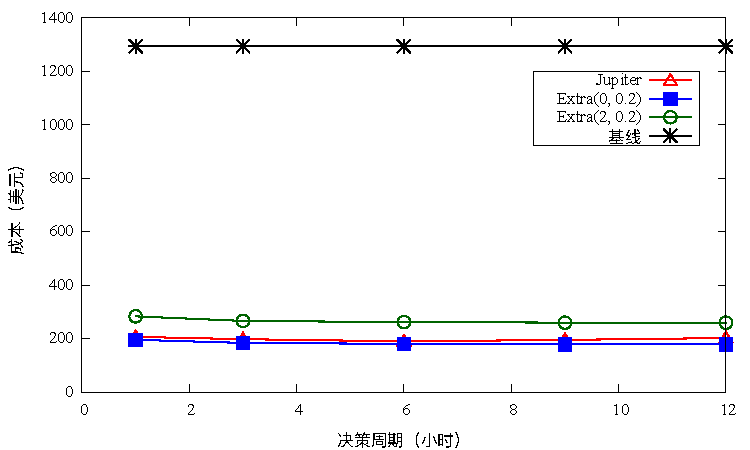
\includegraphics[width=1.0\textwidth]{cost-dss}
  \caption{不同竞价策略下基于纠删码的分布式存储服务的竞价实例租用成本(2014年10-12月)}
  \label{figure:dsscost}
\end{figure}
\begin{figure}
  \centering
  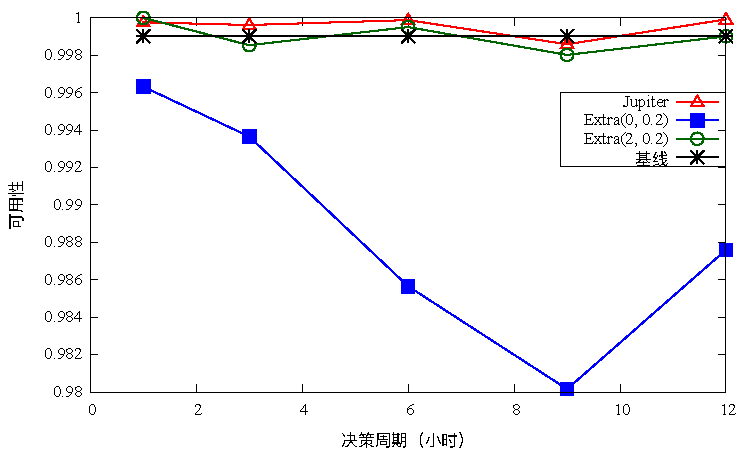
\includegraphics[width=1.0\textwidth]{ava-dss}
  \caption{不同竞价策略下基于纠删码的分布式存储服务的可用性(2014年10-12月)}
  \label{figure:dssavailability}
\end{figure}

Jupiter竞价框架除竞价周期为9个小时的配置均保证了和基线相当的服务可用性级别。在竞价周期为9个小时的配置下,分布式存储服务的失效时间略长于可用性级别的要求。与之相比,启发式策略 $Extra(0, 0.2)$ 虽成本略低但服务的可用性级别完全处于不可接受的程度。而启发式策略 $Extra(2, 0.2)$ 虽然在可用性相比 $Extra(2, 0.2)$ 策略有所改善,接近 Jupiter 的竞价策略。但 $Extra(2, 0.2)$ 策略所需成本远远高于 Jupiter 的竞价策略。详细评测结果参见图 \ref{figure:dlscost} 和 \ref{figure:dssavailability}。

在图\ref{figure:dlscost} 和 \ref{figure:dsscost}中,本文提出的竞价框架所需成本随不同的竞价周期变动很大。一个短的竞价周期意味着更频繁的申请、启动新的竞价实例会消耗更多的启动时间,进而减少了有效的运行时间增加了计算成本。然而一个很长的竞价周期配置则失去了一些根据市场价格变化改变竞价的机会,因为出于保证服务可用性的考虑对于长竞价周期竞价框架给出的竞价会更高。6小时的竞价周期设置似乎是几个竞价周期中变现最好的。针对Jupiter竞价框架的一个扩展是检测竞价实例市场价格的波动频率并针对性地调整竞价周期。

评测中用于对照的启发式策略是简单和固化的。在没有各个可用区竞价实例市场价格历史数据知识的情况下,笼统的在市场价格基础上增加一个相同的比例作为竞价是过于粗放的。另外,这样的策略由于没有对竞价实例失效概率的估计也无法保证分布式服务的可用性级别。额外的新增竞价实例和一定程度的溢价比例减少了潜在的服务失效,但也显著的增加了成本。总之,这类简单易想的方法不能同时大量节省成本并保证服务的可用性。而Jupiter竞价框架则可以做到成本和可用性感知,在保证可用性的同时大大减少了成本。

\section{本章小节}
\label{sec:jupiter-conclusion}
本章力图解决使用云平台的竞价实例构建分布式服务时如何通过竞价保证服务可用性的问题。文中指出了使用竞价实例时保证分布式系统可用性级别的挑战,系统可用性的分析因为竞价实例失效模型的不同而变得复杂。竞价不足失效是竞价实例的主要失效原因,这完全不同于传统分布式系统中的节点失效。为预测竞价实例的失效概率,文中引入了半马尔可夫链模型来描述竞价实例市场价格的变动。使用竞价实例的分布式系统的可用性据此可通过节点失效概率估测,而不是可同时容忍的最多失效节点数。通过竞价保证可用性的问题进而被形式化为一个非线性规划问题。优化目标是最小化使用竞价实例的成本,关键约束表达了分布式服务的可用性要求。然而,解这样一个非线性规划问题是NP难的。类似穷举搜索的方法完全无法在实际情况中使用。本章描述了一个用于在云平台中使用竞价实例部署高可用分布式服务的竞价框架,并提出了一个可用于实际生产环境的接近最优解的基于枚举和贪心策略的竞价算法。两个基础的分布式服务,分布式锁服务和基于纠删码的分布式存储服务被用于验证竞价框架的有效性。我们的竞价框架针对分布式锁服务和存储服务在保证同使用按需实例部署的同一服务相同的可用性级别的前提下可减少81.23\% 和 85.32\% 的计算成本。
